\chapter{Background}
With respect to the Sun, our planet is moving through space at 30 kilometers per second. Many other objects orbit the sun, and those orbits can overlap or nearly overlap Earth's. The vast majority of these objects are small and are difficult to detect. These objects are known as near-Earth objects. Near-Earth objects consist of many similar rocks, but they have important differences between them. Regardless, they are hazards of the solar system, so we use systems such as all-sky cameras to detect them and gather data about their population distribution.

\section{Asteroids and Meteoroids}
There are five terms that are often incorrectly used interchangeably to describe rocks from space. They are the following: asteroid, meteoroid, meteor, meteorite and fireball. They are visually represented in Figure~\ref{fig:neos}. Compositionally, asteroids and meteoroids are the same. They are composed of rock or metal and travel through space outside Earth's atmosphere. They are delineated by their size.  In order to be defined as a meteoroid, the piece of rock should be at least \mbox{100 $\mu$m}\footnote{Anything smaller than this is nothing more than dust, which makes up the interplanetary dust cloud.}\cite{Steel1996}. The accepted upper boundary on what constitutes a meteoroid but not an asteroid is around 10 meters. Asteroids are much larger, such as the asteroid that caused the Chicxulub crater in the Yucatan peninsula \cite{Bottke2007}. It should be noted that a comet does not belong with these terms as only a small percentage of a comet's composition is rock: it is a mass of ice and dust. 

In terms of their origins, meteoroids are often fragments of asteroids that are separated by some sort of collision in space, or are small pieces of rock and dust that are left behind by comets. Near-Earth asteroids are most likely objects expelled from the main asteroid belt between Mars and Jupiter due to Yarkovsky thermal forces or secular resonances \cite{Bottke2007}. The Yarkovsky thermal force is a net force that occurs from the heating up of one side of an asteroid or meteoroid from the sun. The hotter side dissipates more energy while it cools than the already cold side, and thus that departing energy results in a recoil force moving the asteroid in the direction opposite the hotter side \cite{Bottke2006}. Secular resonance is when an asteroid syncs its precession to a nearby planet. This disturbs the orbit of the asteroid, and causes it to slowly change its orbital eccentricity as a result \cite{Moons1995}.

\begin{figure}[ht!]
  \centering
  \includegraphics[scale=.2]{neos.png}
  \caption{A visual representation of the different varieties of rock in the space near Earth (Photo courtesy of Dr. Jed Rembold).}
  \label{fig:neos}
\end{figure}


\section{Fireballs and Meteors}

Asteroids and meteoroids are by definition only found outside the atmosphere of the planet. They becomes meteors only when they enter the atmosphere. Some literature even rechristens their status from near-Earth objects to inside-Earth objects, or IEOs for short \cite{Bottke2007}. Fireballs are especially bright meteors, and are often chosen to be studied due to their comparatively easy detection. Technically, fireballs are only considered such if they are brighter than Venus, with a magnitude of around -4, but the colloquial use is much less stringent \cite{Harbaugh2008}. 

Most of the time, meteors are completely destroyed as they travel through the atmosphere. This is done through ablation due to how they interact with molecules in the atmosphere. As the meteor hits the molecules in the atmosphere, ionization occurs. The point in the atmosphere at which light is emitted varies based on the velocity of the object. Slower objects need to be in a denser part of the atmosphere before ablation can occur. The average point at which this happens is most often between 70 and 110 kilometers above sea level \cite{Halliday1996}. During this process the meteor loses mass and energy in the form of light. The percentage of energy converted to life is known as the luminous efficiency and is an important term in predicting the mass of a meteor from its luminosity. If there is still mass remaining by the time it comes into contact with the Earth, it cools and becomes a meteorite. More often than not, however, meteors are vaporized tens of kilometers above sea level \cite{Halliday1996}.

Meteors tend to appear during two types of events. The first event is a meteor shower and can be reliably predicted. This is due to Earth going through parts of space where known debris are located. The debris are trails left behind by comets. The majority of these comet trails are due to water vapor drag. As a comet moves around the sun, different parts of its ice evaporate, freeing the small pieces of rock that were embedded inside it \cite{Whipple1951}. A meteor shower can also be caused by a large amount of debris left behind when a comet is fragmented in space \cite{Jenniskens2006}. Many meteor showers are well charted and known at this point. As of this writing there are 112 established meteor showers, with the potential of hundreds more \cite{RRudawskaZKanuchova2017}. Besides a meteor shower, the other event is a single isolated event, called a sporadic event. A sporadic event may have originally been part of a meteor shower or an asteroid belt before getting set off course due to extraneous forces.

\section{Near-Earth Objects}
While there are differences between the types of near-Earth objects, they all share one thing in common: they pose a hazard to any sort of human structure sent out into space. Having more accurate and complete data on the population of these objects will give humanity a better chance to adequately defend these structures and shelters as well as more accurately estimate their lifespans. As space exploration develops, this will become more relevant, with potential landing spots for humans on the Moon and on Mars not having the luxury of the protective atmosphere of Earth. This can be seen just by looking up at the night sky; the moon is pockmarked with craters. This is not just exclusive to the moon, as craters can be seen on any rocky space object that does not have a thick atmosphere. These craters are the most obvious pieces of evidence of meteor strikes The moon also provides another strong example of the power of these strikes, as when a meteoroid hits the lunar surface, enough energy is released as to be visible from Earth \cite{Rembold2015}. Without the protective atmosphere, near-Earth objects could potentially wreak havoc on any structures. For example, the European Space Agency communication satellite Olympus was permanently decommissioned due to damage sustained during the Perseid meteor shower of 1993. The majority of international and national organizations\footnote{These include, but are not limited to, the United Nations, the United States Congress, the European Council, the UK Parliament, the IAU, OECD, NASA, and ESA\cite{Bottke2007}} concerned with planetary protection have all deemed large near-Earth objects to be credible threats to Earth and to any missions out of its atmosphere\cite{Bottke2007}.

Observational data from many different studies has resulted in a model for the population distribution of these objects. Specifically, there is a well-known linear relationship between the mass of an asteroid and the number that exist if plotted along log-log axes \cite{Rembold2015}. This is shown in Figure \ref{fig:population}.

\begin{figure}[ht!]
  \centering
  \includegraphics[scale=.5]{population.png}
  \caption{The population distribution of near-Earth objects is straightforward: small objects are often much more likely than large objects \protect\cite{Rembold2015}.}
  \label{fig:population}
\end{figure}

Initially this model seems reassuring. The larger objects, which would have the most  potential to cause damage, are much less common than the smaller, less energetic objects. The smaller objects would have less energy as 
\begin{equation}
	\textrm{Kinetic Energy} = \frac{mv^2}{2}
	\label{eq:ke}
\end{equation}
where $m$ is equal to the mass and $v$ is equal to the velocity of the object. However, these small objects still pose a large threat to structures due to their extremely fast velocities. A one-millimeter meteoroid has similar strength to a 22-caliber bullet, while a one centimeter meteoroid can be as powerful as a cannonball. This is because velocity is the dominant term in equation \ref{eq:ke} and meteoroid speeds can range from 11 to 70 kilometers per second \cite{Harbaugh2008}. Figure \ref{fig:damage} shows the damage that a pebble-sized object can do to a thick slab of metal, and satellites without armor are much more fragile than that.

\begin{figure}[ht!]
  \centering
  \includegraphics[width=10cm]{damage.jpg}
  \caption{Even small objects such as this ball bearing can exert tremendous amounts of force if they are traveling at 50 kilometers per second \protect\cite{ESA2017}.}
  \label{fig:damage}
\end{figure}


It should be noted that while this model appears consistent, and it may very well be, it is not guaranteed. With such a high population of smaller-sized objects, any variance could greatly change the likelihood of accurately accounting for potential damage. For instance, a satellite can only take so many impacts with meteoroids before becoming disabled. Even if there are only slightly more meteoroids than currently predicted, the lifespan of that satellite would be shortened, jeopardizing missions. 

\section{Detecting Fireballs}
There are many current projects aimed at collecting optical data about meteors \cite{Jenniskens2011,Trigo-Rodriguez2007,Halliday1996}. Most make use of all-sky cameras. All-sky cameras are CCD cameras that are often utilized as video capture devices, recording either 25 or 30 frames per second depending on its video signal \cite{Molau2005}. An all-sky camera is a camera that provides a view of up to 180$^{\circ}$ of the sky above, producing a circular image, as seen in Figure \ref{fig:skypic}. This allows a clear view of the sky as a whole, allowing for easy identification of constellations. By locating constellations, stars can be identified and objects can have their relative location recorded. 
\begin{figure}[ht!]
  \centering
  \includegraphics[width=10cm]{skypic.png}
  \caption{All-sky cameras feature a 360$^{\circ}$ view of the horizon, providing maximum sky coverage. This is an image from a high resolution color camera \protect\cite{Alcor}.}
  \label{fig:skypic}
\end{figure}

In reality, this view is not quite 180$^{\circ}$, but more often around 140$^{\circ}$ due to the fact that lenses wide enough to take in 180$^{\circ}$ end up just taking in the edges of the all-sky cameras chassis instead. Our own camera is only able to see 140$^{\circ}$ into the sky. Figure \ref{fig:atmosphere} shows how much of the sky is covered.
\begin{figure}[ht!]
	\centering
	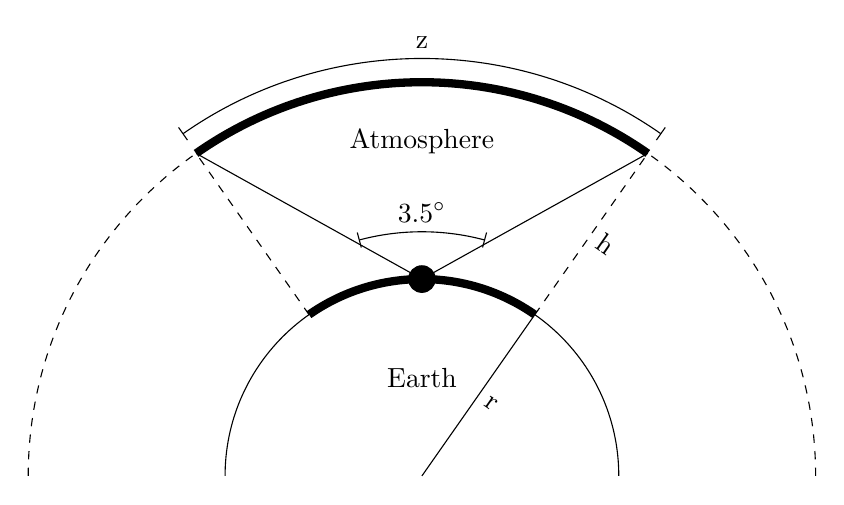
\begin{tikzpicture}
		\draw (0:2.5) arc (0:180:2.5) node at (0,1.25) {Earth};
		\draw[dashed] (0:5) arc (0:180:5) node at (0,4.25) {Atmosphere};
		\draw[] (0,0) -- (55:2.5) node[midway,right,sloped,rotate=270] {r};
%		\draw[dashed] (0,0) -- (125:4);
		\draw (0,2.5) -- (55:5);
		\draw (0,2.5) -- (125:5);
		\draw[dashed] (125:2.5) -- (125:5);
		\draw[dashed]  (55:2.5) -- (55:5) node[midway,right,sloped,rotate=270] {h};
		\draw[line width=3pt] (55:2.5) arc (55:125:2.5);
		\draw[line width=3pt] (55:5) arc (55:125:5);
		\draw[|-|] (55:5.3) arc (55:125:5.3) node[midway,above] {z};
		\draw[|-|] (75:3.1) arc (75:105:3.1) node[midway,above] {$3.5^{\circ}$};
		\fill (0,2.5) circle [radius=5pt];
	\end{tikzpicture}	
	\caption{The all-sky camera can see distance $z$. The area of the Earth it covers are between the points that have the endpoints of $z$ as their zeniths along height $h$. Note that the height of the atmosphere where ablation occurs is often less than 100 kilometers, while the radius of the Earth is 6,371 kilometers, so the radii are not to scale.}
	\label{fig:atmosphere}
\end{figure}
The amount of Earth being covered is defined by taking the edges of the all-sky camera view and treating those as zeniths. A zenith is the point in the sky that is directly above a certain point on Earth. Those points on Earth are the edges of how much of the Earth it covers. Knowing how much of the Earth is covered is useful because those zeniths provide the points where another camera can be placed to overlap one half of the original camera's view of the sky. Overlapping is useful because multiple camera angles allow the triangulation of the object's position and velocity. The amount of sky coverage can be written, using trigonometry, as
\begin{equation} \label{eq:coverage}
	\textrm{Sky Coverage} = \Omega(h+r)^2
\end{equation}
where $\Omega$ is the steradian, $h+r$ is the distance from the center of the Earth to the edge of the area of sky coverage.

Using an average height $h$ of 75 kilometers, the area of the sky that is covered by an all-sky camera such as ours is around 119,000 square kilometers. This is equal to 118,000 square kilometers of land coverage. This is only 0.023 percent of the Earth that is covered, so there is a need for more all-sky cameras to ensure better coverage. Our all-sky camera has been in two locations, Salem and Baker City, Oregon. These two spots provide examples of how much land can be covered in Figure \ref{fig:coverage}. Even for two locations in the same state, there is no overlap.

\begin{figure}[ht!]
	\centering
	\includegraphics[width=10cm]{coverage.png}
	\caption{An all-sky camera can cover a circle with a radius of roughly 200 miles.}
	\label{fig:coverage}
\end{figure}


All-sky cameras are currently detecting fireballs in many places around the world. One notable example is NASA's Camera for All-Sky Meteor Surveillance (CAMS) Network. They have cameras located throughout many parts of the United States, forming a strong cohesive network. The CAMS network has been successful in correctly detecting all known meteor showers\footnote{The meteor showers were the theta Aurigids, chi Taurids, omicron Eridanids, and the supposed iota November Aurigids. The latter was in fact shown to be merely an overlap between the theta Aurigids and chi Taurids with CAMS network data.} during the month of November in 2011\cite{Jenniskens2011}.

NASA is not the only one to have such a network, with other organizations such as the SPanish Meteor Network (SPMN) also possessing well established systems of their own. They were  able to successfully confirm expected meteor showers with the use of their high-resolution, all-sky cameras.\footnote{The meteor showers were the Orionids, the Taurid stream related to comet 2P/Encke, and the delta Aurigids.} They even were able to find the nu Aurigids, that while previously identified, were not expected to be seen \cite{Trigo-Rodriguez2007}. These organizations are able to collect large amounts of data with all-sky camera networks compared to previous endeavors but they do not have enough cameras to come even close to covering the entire sky. Figure \ref{fig:network} shows the Sky Sentinel Camera Network and their coverage in the United States. The network currently operates a network of around 65 cameras and hope to have over 100 in the future \cite{Bannister2012}.

The current model is to have these cameras connected to large structures or buildings with desktop computers where they can access the constant power and internet access that is needed for the detection and analysis. The necessary infrastructure that is currently needed lends these networks to be built in more urban areas, where light and air pollution become more problematic. Therefore this  model also severely limits not only the quantity of skies covered, but also the quality.

\begin{figure}[ht!]
	\centering
	\includegraphics[width=10cm]{network.png}
	\caption{This network manages to cover a lot of area, but it may not have the best observational quality due to the cameras being centered in cities \protect\cite{SkySentinel}.}
	\label{fig:network}
\end{figure}

All-sky cameras themselves are not inherently complex. They are small and can be built relatively cheap, with builds being found online from Sky at Night Magazine and New Mexico State University, among others \cite{Bannister2012}. Figure \ref{fig:schematic} shows the diminutive size of a camera used by the Sky Sentinel network, but also shows the power and video signal cords that have to connect to an external desktop for analysis. 

Having a small, portable system has many potential benefits. Not only does a portable system increase ease of use and decrease equipment cost, it also vastly improves flexibility. For example, if nearby blooming trees block some view of the sky during the spring, a portable system could just be moved, while a permanent system would require the removal of the trees or the acceptance of a less than optimal observational status.

\begin{figure}[ht!]
	\centering
	\includegraphics[width=10cm]{schematic.png}
	\caption{This schematic of an all-sky camera leaves out the attached structure to which the bottom cords must connect\protect\cite{Bannister2012}.}
	\label{fig:schematic}
\end{figure}

Software accompanies all-sky camera systems to perform meteor detections. This saves the user from having to watch hours of video looking for events that may just be a few seconds long. Detection systems look for moving patches of light, and thus can produce numerous false positives from other environmental factors. These include light being reflected off moving clouds and planes flying through the field of vision \cite{Harbaugh2008}. Fortunately, these false positives can mostly be eliminated by visual inspection. The exact setup depends on the specific system, but meteor detection is either constantly processed by a computer checking the frames as they arrive, or the video is stored as a whole to be run through a detection program at a later date \cite{Molau2005}. The software is full-fledged but bulky as a result. For example, METREC is a meteor detection software that is used by networks such as the Polish fireball network. It requires a desktop computer to operate\cite{Molau2005}. The hardware requirements thus require a complete computer to accompany the camera.  

\section{Analyzing Fireballs}

An all-sky camera can result in the acquisition of many pieces of useful information about a meteor. That being said, there are parameters a single all-sky camera cannot extract that a full network can, such as velocity and height. If there is a system of multiple cameras detecting the same meteor the orbit can be extrapolated as well \cite{Trigo-Rodriguez2009}. The Canadian fireball network detected 259 fireballs in 1996, and was able to get values for height, velocity, magnitude and mass for every fireball \cite{Halliday1996}. A single all-sky camera would only be able to get magnitude, and would have to extract mass from that. For a full fireball network, having velocity means it can find the mass with the relationship
\begin{equation} 
	\label{eq:mass}
	\frac{m_d}{A} = -\frac{\rho_a v^2}{2 \dot v}
\end{equation}
where $m_d$ is the mass at a certain point in the flight, $A$ is the cross sectional area at that same point in flight, $\rho_a$ is the atmospheric density, and $v$ is velocity \cite{Halliday1996}.


Not only does the velocity help determine mass in this situation, it also can be used to work backwards to find an estimate of the velocity before the affects of drag began slowing it down. This means that all-sky cameras can be used to gather data on the potential velocities of meteor showers in open space. The SPanish Meteor Network (SPMN) used velocity data to extrapolate such pre-atmosphere velocities with their five station setup in 2006 \cite{Trigo-Rodriguez2007}. 

Ultimately, all-sky cameras are most useful for measuring the photometric qualities of objects in the sky. They can detect fireballs and then provide the needed data to determine the fireballs' magnitudes, which is how bright they appear to the camera. This, however, can be done with just a single all-sky camera.

It should be noted that there are differing techniques when performing photometry. Different cameras are more sensitive to different wavelengths of light, and that can make comparing results from different cameras challenging. One solution to this is to apply a filter. A filter isolates light along a specific wavelength of the electromagnetic spectrum, as shown in Figure \ref{fig:bands}. For example, a visual filter is one that focuses on visible light, being centered on the wavelength for green light. The most commonly used values for star magnitudes are values determined after applying a visual spectrum filter. If a camera is more sensitive towards the infrared spectrum, an R filter would more likely fit its data, and can be applied instead \cite{Suggs2014}. It is possible to compare magnitude values with two different filters, but the process is somewhat convoluted and best to be avoided.

\begin{figure}[ht!]
	\centering
	\includegraphics[width=10cm]{bands.png}
	\caption{The visual filter, outlined in green, is shifted to the left of the R filter, which is towards the infrared part of the spectrum. The black outline is an example of what a camera's sensitivity may look like \protect\cite{Suggs2017}.}
	\label{fig:bands}
\end{figure}

In some cases, it is useful to not apply a filter at all. While this can make it difficult to calibrate the camera to other known values, this guarantees that all light is being detected. This is crucial in highly sensitive detection situations where it would be ill-advised to sacrifice any of the small amount of potential data \cite{Rembold2015}. Even if no filter is applied, knowing the different bands allows the comparison of data to similar observations. For example, if the unfiltered camera sensitivity closely approximates the R band, R filter magnitudes are comparable.

The luminosity can be used to find the mass, but only by using approximations for other values such as density, which can be estimated due to the structural analysis of meteorite collections. As luminosity is the only needed data point, a single all-sky camera is viable for measuring the population distribution.

But how does one get from intensity to luminosity? The relationship between the two is

\begin{equation}
	L = (SA)I,
	\label{eq:luminosity}
\end{equation}
where $L$ is luminosity, $I$ is intensity, and $SA$ is the surface area over which the energy wave has propagated. In order to find the luminosity from intensity, we need to assume that the object radiates energy equally in all directions, forming a sphere. This assumption is not too far off from the actual shape of most meteors. Making this assumption, Equation~\ref{eq:luminosity} becomes 

\begin{equation}
	L_{obs} = 4 \pi r^3 I.
\end{equation}
Now that the intensity is converted to luminosity, that luminosity can then be used to find its total kinetic energy. The relationship between the two is

\begin{equation}
	L = \tau T,
	\label{eq:kinetic}
\end{equation}
where $L$ is again luminosity, $T$ is kinetic energy, and $\tau$ is the luminous efficiency. Again, the luminous efficiency is simply the proportion of a fireball's energy that is dissipated as light. Once the kinetic energy is known, we can relate that to mass, as

\begin{equation}
	T = \frac{v^2}{2}\frac{dm}{dt},
\end{equation}
where $v$ is velocity, $m$ is mass, and $t$ is time. Again, with only one all-sky camera assumptions about the velocity have to be made but as velocities of meteors vary at most by a factor of 2, this assumption does not create problems along the log-log graph of Figure~\ref{fig:population}. Again, this could be easily resolved by having multiple all-sky cameras detect the event. Notice that while the mass of an object is usually treated as constant when calculating kinetic energy, since the entirety of the object's mass is burning up, we can integrate over the entire event to find that original mass. This integral can be written as

\begin{equation}
m =\int \frac{2L}{\tau v^2}\,dt.
\end{equation}
This integration is why the entire light curve of a meteor event needs to be collected. The methods for doing so is described in the next section.
